\section{Auswertung}
\label{sec:Auswertung}
In diesem Kapitel werden alle Mittelwerte und deren Fehler berechnet. 
Dazu wurde Python Numpy benutzt. Diese Mittelwerte sind die anzunehmenden, fehlerbehafteten Größen.

Der Mittelwert:
\begin{center}
  \begin{equation}
    \label{eq:Mittelwert}
  \bar{x}=\frac{1}{n}\sum\nolimits_{i=0} x_i
  \end{equation} 
\end{center}

Die Standardabweichung:
\begin{center}
  \begin{equation}
    \label{eq:standardabweichung}
  
    $\sigma=\sqrt{\frac{\sum(x_i-\bar{x})^2}{n-1}}$
  \end{equation}
\end{center}

Der Fehler des Mittelwertes:
\begin{center}
  \begin{equation}
    \label{eq:mittelwertfehler}
    \sigma_{\bar{x}}=\frac{\sigma}{\sqrt{n}}
  \end{equation}

  
\end{center}

Die Gaußsche Fehlerfortpflanzung:
\begin{center}
\begin{equation}
  \label{eq:gaussfehler}  
\sigma_x=\sqrt{(\frac{\partial f}{\partial x_1})^2\sigma_{x_1}^2+(\frac{\partial f}{\partial x_2})^2\sigma_{x_2}^2+...+(\frac{\partial f}{\partial x_n})^2\sigma_{x_n}^2}
\end{equation}
\end{center}
\subsection{Abmessungen und Spezifikationen der Proben}
\label{sec:abmessungen}
\subsubsection{Abmessungen Draht}
\label{sec:abmessungenDraht}
Bei der ersten vermessenen Probe handelt es sich um einen Kupferdraht mit folgenden Werten:
\begin{center}
    Länge: $L_D=\SI{1,37}{m}$\\
    Durchmesser: $d_D=1,05\pm0,01 \times 10^{-4} m$\\
    Wiederstand: $R_D=\SI{2,6\pm0,7}{\Omega}$
\end{center} 
Um den Wert für den Widerstandangeben zu können wurde die Probe in beide Richtungen 
vermessen und der Mittelwert nach \autoref{eq:Mittelwert} mit zugehörigem Fehler nach 
\autoref{eq:mittelwertfehler} berechnet.
\subsubsection{Abmessungen der Folie}
\label{sec:abmessungenFolie}
Die zweite vermessene Probe ist eine Kupferfolie mit diesen Werten:
\begin{center}
    Länge: $L_F=25,0\pm1,0\times 10^{-3} m$\\
    Breite: $b_F=24,0\pm1,0\times 10^{-3} m$\\
    Dicke: $d_F=2,7\pm0,1\times 10^{-5} m$
\end{center} 
\subsubsection{Die Hallspannung}
Für die Folie aus \autoref{sec:abmessungenFolie} lässt sich die Hallspannung ohne Störung mit 
\autoref{eq:hallspannung} berechnen. Es folgt also:


\subsection{Die mikroskopischen Leitfähigkeitsparameter}
\label{sec:leitfaehigkeitsparameter}
In diesem Kapitel sollen einige Größen berechnet werden um die Materialeigenschaften der Probe
auf mikroskopischer Ebene zu spezifizieren.
\subsubsection{Ladungsträger pro Volumen $n$}
\label{sec:ladungstraegerVolumen}
Die Anzahl der Ladungsträger pro Volumeneinheit lässt sich mit \autoref{eq:elektronenzahl} berechen, da 
für unterschiedliche Magnetfeldflüsse unterschiedliche Hallspannungen gemessen werden ergibt sich auch
eine Reihe von Anzahlen für Ladungsträger pro Volumen. Da es aber nur eine korrekte Zahl geben kann wird hier
der Mittelwert nach \autoref{eq:Mittelwert} und dessen Fehler nach \autoref{eq:mittelwertfehler} angeben:
\begin{center}
    $n=6,26\pm0.35 \times 10^{27} \frac{1}{m^3}$
\end{center}
\subsubsection{Ladungsträger pro Atom $z$}
\label{sec:ladungstraegerAtom}
Kupfer hat ein molares Volumen von etwa $7,11 \times 10^{-6} \frac{m^3}{mol}$, daraus folgt das ein
 Kubikmeter etwa $V_m=\SI{14065}{mol}$ enthält. Ein $mol$ hat genau $N_A$ \autoref{sec:Konstanten} Atome.
 Die Anzahl der zur elektrischen Leitung nutzbaren Elektronen pro Atom ergibt sich also aus:
 \begin{center}
     $z=\frac{n}{N_A V_m}$\\
     $\Rightarrow z=0,74\pm0,04 \approx 1$
 \end{center}
 Da z ganzzahlig sein muss wird Kupfer ein nutzbares Elektron pro Atom haben.

\subsubsection{Die mittlere Flugzeit $\bar{\tau}$}
\label{sec:flugzeit}
Aus \autoref{eq:widerstand} folgt für eien Runden Draht mit $Q=\frac{\pi d_D^2}{4}$ sofort:
\begin{equation}
    \label{eq:tau}
    \bar{\tau}=\frac{8m_0L}{e_0^2n R \pi d_{D}^2}
\end{equation}
\begin{center}
    $\Rightarrow \bar{\tau}=(1.79\pm0.11) \times10^{-12} s$
\end{center}

\subsubsection{Die mittlere Driftgeschwindigkeit $\bar{v_d}$}
\label{sec:driftgeschwindigkeit}
Mit \autoref{eq:drift} und $j=1000000\frac{A}{m^2}$:
\begin{center}
    $\bar{v_d}=-\frac{j}{ne_0}$\\
    $\Rightarrow \bar{v_d}=-1,0 \pm 0,06 \times 10^{-3} \frac{m}{s}$
\end{center}
\subsubsection{Die Beweglichkeit $\mu$}
\label{sec:beweglichkeit}
Nach der Rechenvorschrift \autoref{eq:mu} folgt mit dem Ergebnis aus \autoref{sec:flugzeit}:
\begin{center}
    $\mu=0.158\pm0.009 \frac{A^2s^3}{kg} $
\end{center}
\subsubsection{Die Totalgeschwindigkeit v}
\label{sec:totalgeschwindigkeit}
Die totale Driftgeschwindigkeit $\vert v \vert$ ergibt sich mit \autoref{eq:vtot} und dem Ergebnis aus 
\autoref{sec:ladungstraegerVolumen} zu:
\begin{center}
    $\vert v \vert=(6.60\pm0.12)\times10^5 \frac{m}{s}$
\end{center}

\subsubsection{Die mittlere freie Wellenlänge $\bar{l}$}
\label{sec:wellenlaenge}
Die materialspezifische freie Wellenlänge ergibt sich über \autoref{eq:freieWellenlaenge} mit den Ergebnissen 
aus \autoref{sec:totalgeschwindigkeit} und \autoref{eq:tau} zu:
\begin{center}
    $\bar{l}=(1.18+/-0.05)\times 10^{-6} m$
\end{center}
\subsection{Löcher- oder Elektronenleitung}
\label{sec:leiterart}
In diesem Versuch wurde eine Kupferprobe untersucht, Kupfer ist bekanntermaßen ein Elektronenleiter, dies 
zeichnet sich durch eine ausgeprägte Hallspannung aus. Zudem hat die Hallspannung die für eine Elektronenleiter
zu erwartende Richtung.
\subsection{Flussdichte $B$ des verwendeten Magneten}
\label{sec:verwendeterMagnet}
Der für die Messungen benutzte Elektromagnet wurde bezüglich der Feldstärke im Spalt des Eisenkernes vermessen.
Dazu wurde ein Teslameter in diesen Spalt gehalten und der Spulensrom $I$ in $\SI{0,5}{A}$ bis zur maximalen Leistung 
der angeschlossenen Konstantstromquelle erhöht, anschließend wurde umgepolt und der Prozess wurde wiederholt. 
In diesem Diagram \autoref{fig:magnet} sind ist der Spulenstrom $I$ gegen die daraus resultierende 
Flussdichte $B$ aufgetragen:
\begin{figure}
    \centering
    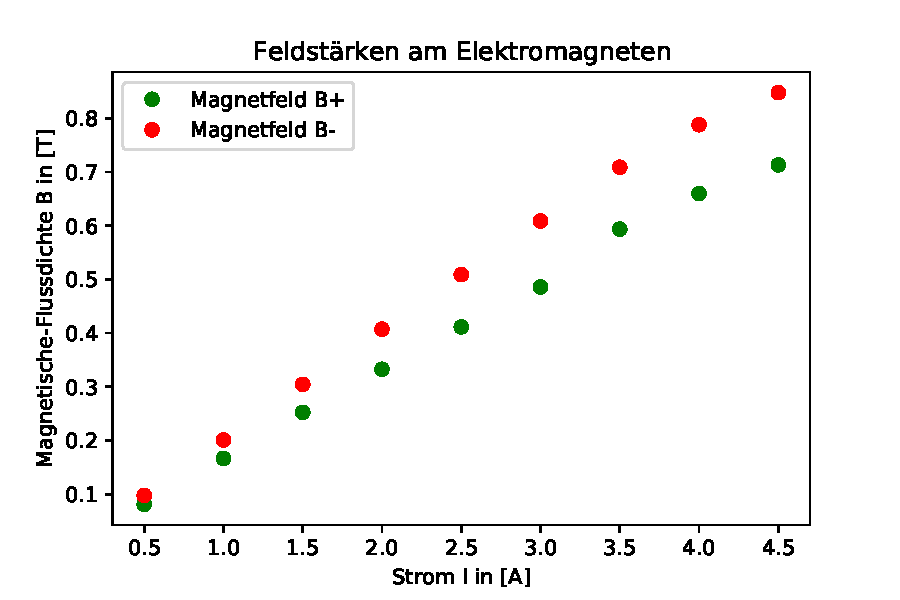
\includegraphics{plot.pdf}
    \caption{Flussdichte im Elektromagneten}
    \label{fig:magnet}
  \end{figure}

